%\pdfoutput=1
% Uncomment line above if submitting to arXiv and using pdflatex

% $Id: main.tex 97873 2016-09-08 18:28:41Z michaelt $
% ============================================================================
% Purpose: Template for LHCb documents
% Authors: Tomasz Skwarnicki, Roger Forty, Ulrik Egede
% Created on: 2010-09-24
% ============================================================================
\documentclass[12pt,a4paper]{article}
%%\documentclass[12pt,letter]{article}
% For two column text, add "twocolumn" as an option to the document
% class. Also uncomment the two "onecolumn" and "twocolumn" lines
% around the title page below.

% Variables that controls behaviour
\usepackage{ifthen} % for conditional statements
\newboolean{pdflatex}
\setboolean{pdflatex}{true} % False for eps figures

\newboolean{articletitles}
\setboolean{articletitles}{true} % False removes titles in references

\newboolean{uprightparticles}
\setboolean{uprightparticles}{false} %True for upright particle symbols

\newboolean{inbibliography}
\setboolean{inbibliography}{false} %True once you enter the bibliography

% THis file contains all the default packages and modifications for
% LHCb formatting

%% %%%%%%%%%%%%%%%%%%
%%  Page formatting
%% %%%%%%%%%%%%%%%%%%
%%\usepackage[margin=1in]{geometry}
\usepackage[top=1in, bottom=1.25in, left=1in, right=1in]{geometry}

% fallback for manual settings... uncomment if the geometry package is not available
%
%\voffset=-11mm
%\textheight=220mm
%\textwidth=160mm
%\oddsidemargin=0mm
%\evensidemargin=0mm

\columnsep=5mm
\addtolength{\belowcaptionskip}{0.5em}

\renewcommand{\textfraction}{0.01}
\renewcommand{\floatpagefraction}{0.99}
\renewcommand{\topfraction}{0.9}
\renewcommand{\bottomfraction}{0.9}

% Allow the page size to vary a bit ...
\raggedbottom
% To avoid Latex to be too fussy with line breaking ...
\sloppy

%% %%%%%%%%%%%%%%%%%%%%%%%
%% Packages to be used
%% %%%%%%%%%%%%%%%%%%%%%%%
\usepackage{microtype}
\usepackage{lineno}  % for line numbering during review
\usepackage{xspace} % To avoid problems with missing or double spaces after
                    % predefined symbold
\usepackage{caption} %these three command get the figure and table captions automatically small
\renewcommand{\captionfont}{\small}
\renewcommand{\captionlabelfont}{\small}

%% Graphics
\usepackage{graphicx}  % to include figures (can also use other packages)
\usepackage{color}
\usepackage{colortbl}
\graphicspath{{./figs/}} % Make Latex search fig subdir for figures

%% Math
\usepackage{amsmath} % Adds a large collection of math symbols
\usepackage{amssymb}
\usepackage{amsfonts}
\usepackage{upgreek} % Adds in support for greek letters in roman typeset

%% fix to allow peaceful coexistence of line numbering and
%% mathematical objects
%% http://www.latex-community.org/forum/viewtopic.php?f=5&t=163
%%
\newcommand*\patchAmsMathEnvironmentForLineno[1]{%
\expandafter\let\csname old#1\expandafter\endcsname\csname #1\endcsname
\expandafter\let\csname oldend#1\expandafter\endcsname\csname
end#1\endcsname
 \renewenvironment{#1}%
   {\linenomath\csname old#1\endcsname}%
   {\csname oldend#1\endcsname\endlinenomath}%
}
\newcommand*\patchBothAmsMathEnvironmentsForLineno[1]{%
  \patchAmsMathEnvironmentForLineno{#1}%
  \patchAmsMathEnvironmentForLineno{#1*}%
}
\AtBeginDocument{%
\patchBothAmsMathEnvironmentsForLineno{equation}%
\patchBothAmsMathEnvironmentsForLineno{align}%
\patchBothAmsMathEnvironmentsForLineno{flalign}%
\patchBothAmsMathEnvironmentsForLineno{alignat}%
\patchBothAmsMathEnvironmentsForLineno{gather}%
\patchBothAmsMathEnvironmentsForLineno{multline}%
\patchBothAmsMathEnvironmentsForLineno{eqnarray}%
}

% Get hyperlinks to captions and in references.
% These do not work with revtex. Use "hypertext" as class option instead.
\usepackage{hyperref}    % Hyperlinks in references
\usepackage[all]{hypcap} % Internal hyperlinks to floats.

%\input{lhcb-symbols-def} % Add in the predefined LHCb symbols

% Make this the last packages you include before the \begin{document}
\usepackage{cite} % Allows for ranges in citations
\usepackage{mciteplus}

\usepackage{longtable} % only for template; not usually to be used in PAPERs

\begin{document}

%%%%%%%%%%%%%%%%%%%%%%%%%
%%%%% Title     %%%%%%%%%
%%%%%%%%%%%%%%%%%%%%%%%%%
\renewcommand{\thefootnote}{\fnsymbol{footnote}}
\setcounter{footnote}{1}


% %%%%%%% TITLE PAGE--------
% Author: Dónal Murray
% Based on LHCb-PAPER journal paper title page template
% Created May 2017

%%%%%%%%%%%%%%%%%%%%%%%%%
%%%%%  TITLE PAGE  %%%%%%
%%%%%%%%%%%%%%%%%%%%%%%%%
\begin{titlepage}
\pagenumbering{roman}

% Header ---------------------------------------------------
\vspace*{-1.5cm}
\centerline{\large }
\vspace*{1.5cm}
\noindent
\begin{tabular*}{\linewidth}{lc@{\extracolsep{\fill}}r@{\extracolsep{0pt}}}
  & & \\
  & & \today \\ % Date - Can also hardwire e.g.: 23 March 2010
  & & \\
\end{tabular*}

\vspace*{4.0cm}

% Title --------------------------------------------------
{\normalfont\bfseries\boldmath\huge
\begin{center}
  AC circuit impedence calculator\\
  \vspace*{0.5cm}
  \large{Object Oriented Programming final project}
\end{center}
}

\vspace*{1.0cm}

% Authors -------------------------------------------------
\begin{center}
D\'onal Murray \\
{\normalfont\itshape\small
Student ID: 8381250\\
}
\bigskip
{\normalfont\itshape\small
University of Manchester, Manchester, United Kingdom\\
}
\end{center}

\vspace{\fill}

% Abstract -----------------------------------------------
\begin{abstract}
  \noindent
  A program is presented for the manipulation and storage of alternating current circuits. Series and parallel circuits can be constructed using an arbitrary number of resistors, capacitors, inductors or other circuits composed of the listed components. Impedences of all components in the circuit as well as the total impedence of the circuit are calculated and circuits diagrams can be printed. The program allows the user to save the current project to a file and load old projects from a file. The program is designed to fully comply with the current \CC{} standard and to make use of advanced features of object oriented programming included in \CC11.
\end{abstract}

\vspace*{1.0cm}

\begin{center}

\end{center}

\vspace{\fill}

{\footnotesize
\centerline{
}}
\vspace*{2mm}

\end{titlepage}

%%%%%%%%%%%%%%%%%%%%%%%%%%%%%%%%
%%%%%  END OF TITLE PAGE  %%%%%%
%%%%%%%%%%%%%%%%%%%%%%%%%%%%%%%%

%  empty page follows the title page ----
\newpage
\setcounter{page}{2}
\mbox{~}

\cleardoublepage

% %%%%%%%%%%%%% ---------

\renewcommand{\thefootnote}{\arabic{footnote}}
\setcounter{footnote}{0}

%%%%%%%%%%%%%%%%%%%%%%%%%%%%%%%%
%%%%%  Table of Contents  %%%%%%
%%%%%%%%%%%%%%%%%%%%%%%%%%%%%%%%
%%%% Uncomment next 2 lines if desired
%\tableofcontents
%\cleardoublepage


%%%%%%%%%%%%%%%%%%%%%%%%%
%%%%% Main text %%%%%%%%%
%%%%%%%%%%%%%%%%%%%%%%%%%

\pagestyle{plain} % restore page numbers for the main text
\setcounter{page}{1}
\pagenumbering{arabic}

%% Uncomment during review phase.
%% Comment before a final submission.
%\linenumbers

\section{Introduction}
\label{sec:introduction}
This report aims to outline the design and implementation of a program written in \CC{} to calculate the impedence of AC circuits consisting of any number of ideal resistors, capacitors and inductors in series or parallel. The program attempts to make best use of the advanced idiomatic features of \CC.

%C++ intro
\CC{} is an object oriented programming language that was created by Bjarne Stroustrup in 1983, initially with the aim to introduce object oriented programming into C~\cite{ref:} but which has since diverged to become a programming language in its own right and one of the most popular programming languages in the world~\cite{ref:}.

Object oriented programming is centred around classes and their instantiations called objects which contain data and functions which can be either public, allowing the data or function to be accessed from outside of the class, or private, allowing access only within a specified scope. There is a third classification, protected, which will be discussed in section~\ref{sec:code}.

\subsection{AC circuit theory}
In contrast with DC circuit theory, where the current through a circuit is opposed only by the resistance, $R$, of that circuit, in AC circuit theory the current through an AC circuit is opposed by a combination of both the resistance and reactance, X and their combination is called the impedance, Z. Whereas resistance is the opposition to the flow of current, the reactance is the opposition to the \textit{change} in flow of current. This is why the reactance of components is irrelevant with DC circuits, as the current through the circuit is not changing.

\subsubsection*{Impedance}

Mathematically when dealing with AC circuits, complex numbers are used for the impedance with the real part representing the resistance and the imaginary part representing the reactance such that

\begin{equation}
  Z=R+jX ,
\end{equation}

where, to agree with convention, $j = \sqrt{-1}$ is used in place of $i$ to avoid confusion with the current which is conventionally denoted $I$.
The program is designed to make all of its calculations with ideal components, which means that a resistor only has resistance and zero reactance and that inductors and capacitors only have reactance and zero resistance. Therefore assuming ideal components, the impedance of a capacitor, inductor and resistor can be found using

\begin{align}
  Z_{C}&=\frac{1}{j\omega{}C},   &   Z_{L}&=j\omega{}L,   & \textnormal{and} & &   Z_{R}&=R
\end{align}

respectively, where $\omega$ is the angular frequency of the AC current and $C$ and $L$ are the capacitance and inductance respectively.

With $n$ components connected in series, the total impedance can be found by taking the sum of the impedances of the constituent components with

\begin{equation}
  Z_{total} = Z_1 + Z_2 + \ldots + Z_n
\end{equation}

and with $n$ components connected in parallel, the inverse of the total impedance can be found by taking the sum of the inverse of the impedances of the constituent components with

\begin{equation}
  \frac{1}{Z_{total}} = \frac{1}{Z_1} + \frac{1}{Z_2} + \ldots + \frac{1}{Z_n}
\end{equation}

which requires the conjugate and modulus to be found for each of the complex impedances, which is discussed in section~\ref{sec:code}.

\subsubsection*{Phase difference}
%fact check this
By plotting the impedance on the complex plane, the resulting plot is called a phasor diagram~\cite{} and can be used to determine the phase difference, which describes the offset between the voltage and the current. The phase difference is found by taking the argument of the impedance. Capacitors have a phase difference of $-90\degree$ which means that the voltage lags the current by $90\degree$ and inductors have a phase difference of $90\degree$ which means that the voltage leads the current by $90\degree$


\section{Code design and implementation}
\label{sec:code}
\CC{} -- abstraction, encapsulation, inheritance and polymorphism


Instead of making separate classes for capacitors, inductors and resistors, an abstract base class was made which functions as an interface for all three. The RCL classes then inherit from this class This abstract base class, \verb!Component!, contained a virtual function prototype \verb!get_impedance! which is


\CC{} allows programs to be broken up into multiple files in a bid to reduce the number of lines per file and make the code more readable and more straightforward for the programmer to edit. Separating classes into a separate file allows for modularity; that is the ability to reuse the same classes for different programs.
A further feature of this modularity is the ability to separate the interface of each class from its implementation. By separating the interface into a header file (many conventions exist for the naming of \CC{} header files but this project exclusively uses the \verb!.h! extension) and consists of the class definition in which the member data are declared and the member functions are prototyped. Header files are included (with the \verb!#include "*.h"! preprocessor directive) but not compiled, whereas source files are compiled but not included. The implementation was contained in files with the \verb!.cpp! extension, but like header files, many other naming conventions exist.


In the design of this project, the code was split into seven header files which contained class definitions, namespace and seven source files which are listed along with a short description of their contents.

\begin{figure}
  \begin{center}
    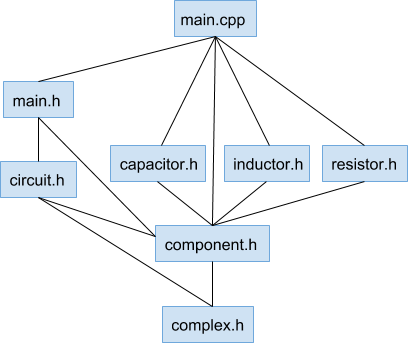
\includegraphics[width=.5\textwidth]{hierarchy}
  \end{center}
  \caption{The hierarchy of header files showing the main file at the top and the chain of its dependencies leading down.}
  \label{fig:hierarchy}
\end{figure}

%\subsection{\CC{} concepts}








prototyping functions\\

vectors\\
smart pointer\\
lambdas\\
namespaces and binary scope operator\\
function template\\
static data\\


\section{Results}
\label{sec:results}
(illustrates how code is used including input and output details)


\section{Discussion and Conclusions} % (3 pages)
\label{sec:discussion}
(include discussion of how code could be improved/extended beyond project)


\addcontentsline{toc}{section}{References}
\setboolean{inbibliography}{true}
\bibliographystyle{LHCb}
\bibliography{oop}

\end{document}
